%preamble
\documentclass[letterpaper]{article}
\synctex=1

\usepackage{listings}
\lstset{
%language=Assembler
% breaklines=true
%frame=single,
%xleftmargin=-1pt
}
\usepackage{geometry}
\usepackage{array}
\usepackage{lipsum}

\usepackage{graphicx}
\usepackage{float}
\graphicspath{ {images/} }

\usepackage{float}

% \usepackage[section]{placeins}
%
% \newenvironment{changemargin}[2]{%
% \begin{list}{}{%
% \setlength{\topsep}{0pt}%
% \setlength{\leftmargin}{#1}%
% \setlength{\rightmargin}{#2}%
% \setlength{\listparindent}{\parindent}%
% \setlength{\itemindent}{\parindent}%
% \setlength{\parsep}{\parskip}%
% }%
% \item[]}{\end{list}}

% \usepackage{tabu}
%actual document
\begin{document}

  %titlepage
  \begin{titlepage}
    \begin{center}

      \LARGE
      ECE 212 Lab - Introduction to Microprocessors

      Department of Electrical and Computer Engineering

      University of Alberta

      \vspace{2cm}

      Lab 1: Introduction to Assembly Language.

      \vspace{5cm}
      \Large

      \begin{tabular}{ | m{5cm} | m{5cm} | }
        \hline
        Student Name & Student \\
        \hline
        Arun Woosaree & xxxxxxx \\
        \hline
        Navras Kamal & 1505463 \\
        \hline
      \end{tabular}


      % \begin{tabu} to 0.8\textwidth{  | X[c] | X[c] | }
      %   \hline
      %   Student Name & Student \\
      %   \hline
      %   Arun Woosaree & xxxxxxx \\
      %   \hline
      %   Navras Kamal & 1505463 \\
      %   \hline
      % \end{tabu}


    \end{center}
\end{titlepage}

%table of tableofcontents

\tableofcontents

% \vfill
\newpage

\section{Introduction}
\textbf{TODO
  This text is filler text from an ece 210 lab report}
  The purpose of this lab is to learn and test with the Assembly language in a hands on environment
  in order to solidify the concepts learned in class and to improve our skill in the language.  In
  addition we will be learning how to handle the Netburner ColdFire boards directly, manipulating
  the contents of their memory and data structures.  Finally we are going to learn how to work inside
  the Eclipse IDE environment and how to properly use the powerful tools that come alongside it.  

  The code will be developped for the Netburner ColdFire Platform, which has some parameters that should
  be kept in mind throughout testing.  There is multiple Data and Address registers, and the memory can
  is indexed by hexadecimal codes.  The data and the stored locations can each be modified directly, values
  can be compared and the code can branch into different sections depending on the values of the CCR bits,
  which store information about the outcome from the last comparison or valid operation, such as if a 
  value is negative or zero.  These will be used to execute code conditionally.  

  The lab will be split into two sections, each with a different goal but with similar implementation.
  For one part we will be taking in an ASCII value and if the character it represents is a character
  included in the symbols for hexadecimal numbers then that hexadecimal value is output, otherwise
  it returns an error.  For the second part an ASCII value is taken in, and if the character it represents
  is a letter in the English language (A-Z) then the ASCII code for the character in the opposite case 
  is output.  Thus valid uppercase english letters are converted to their lowercase equivalents in ASCII 
  and vice versa.  

  These experiments will introduce the general programming practices of loops, if - then - else statements, 
  and the manipulation of stored data.  More specifically to Assembly this will introduce the movement of
  memory and data to and from different parts of the Netburner chip, using techniques such as referencing
  memory addresses and copying data to local data registers.  The debugger tools of the IDE will be used
  to closely examine this movement and to analyze all changes to the data in order to solve issues in 
  development as well as to test the code.  This is all building off the concepts explored in Lab 0. 
  
  They will also introduce the computing science practice of Pair Programming, wherein two people work on 
  one computer to develop and test code in tandem.  The partners are divided into the Driver and the Navigator.
  In this structure the Driver is the one responsible for the physical typing of the code into the computer,
  and the Navigator reviews this code and clarifies the meaning of each passage in order to find bugs faster
  and to improve efficiency in testing.  The two partners should communicate constantly and switch in order
  to maximize the efficiency of this working model.  This will not only decrease time needed for development
  but it will also improve the quality of code from each partner.  


\section{Design}
  \subsection{Part A}
    For the first part of the lab, the address register a1 was chosen to initially point to
    memory location 0x2300000, which is the starting point of where the input data was stored.
    We used this address register to keep track of the memory location of the next long word
    of data to be read as an input to our program. Even though one memory location is capable
    of storing one ASCII character, in this lab, 4 memory locations were used to store one
    ASCII character, as specified in the lab manual.
    Next, a2 was selected to initially point at the memory location 0x231000, which is the
    starting location of where our output for the converted values was. This register
    was used to keep track of the memory location of where the next long word of
    our converted data would go. The data register d2 was chosen to temporarily store
    data so we could do comparisons and process the input data.
    The \textit{Setzeros.s} and the \textit{DataSrorage.s}
    files, which were provided, were used to initialize memory contents.

    We started with a loop branch that served as our main looping function. This
    loop first starts by moving data from a memory location pointed to by a1, to
    the data register d2 so that we could start comparing the input data to known ASCII values.
    In the first comparison, the input character is compared to `0x0D', which is the ASCII
    code for the `Enter' key. This code is meant to signal the end of the program, so if
    the input was the ASCII code for `Enter', we branched to a label that
    would end our program. The next step was to determine if the input character was valid.
    For Part A, an input character was valid if it was an ASCII character from 0-9, A-F, or a-f.
    In other words, the data was accepted if it was in the following ranges: 0x30-0x39,
    0x41-0x46, or 0x61-0x66. If the input character was invalid, we brached to a label
    named `err', which would put the error code `FFFFFFFF' in the memory location
    pointed to by a2, which keeps track of where our output data goes.

    If the input character was valid, we had three branches to take care of each
    of the accepted ranges of input. For example, in the branch that took care of the
    input range A-F, the ASCII value of `A' was subtracted from the input value, and
    the difference was added to the hex value 0xA. The converted value is then moved
    to the memory location pointed to by a2, which keeps track of where our output data goes.
    Similar steps were done to convert input characters in the other accepted ranges.
    After converting the input character and moving the output to the location pointed by a2,
    we branched to a label `endloop', which increments the addresses stored in a1 and a2 by 4,
    and then branches to the loop, where the process is repeated. The flowchart diagram can
    be found in the Appendix.

    % \begin{figure}
    %   \includegraphics{/path/to/figure}
    %   \caption{}
    %   \label{}
    % \end{figure}

    \subsubsection{Part A Sample Calculations of Conversion}

        input = `9' = 0x39\\
        0x39 - 0x30 = 0x9\\
        \\
        input = `E' = 0x45\\
        0x45 - 0x41 = 0x4\\
        0x4 + 0xA = 0xE\\
        \\
        input = `d' = 0x64\\
        0x64 - 0x61 = 0x3\\
        0x3 + 0xA = 0xD



  \subsection{Part B}
    The design for Part B was very similar to Part A. The address register a1 still
    initially points to 0x2300000, but this time, a2 now points to 0x2320000, which is
    where the converted data is stored.The same data register d2 was used to temporarily
    store the input and process the data. Just like in Part A, the \textit{Setzeros.s} and the \textit{DataSrorage.s} files
    were used to initialize memory contents as well.

    Once again, we had a loop branch that initially loads input data from the location
    pointed to by a1 into data register d2, and the ASCII `Enter' code still terminates
    the program, as before. In Part B, valid inputs are the ASCII characters A-Z and a-z.
    (0x41-0x5A and 0x61-0x7A)
    Error handling was also similar to Part A, where the value 0xFFFFFFFF was stored at the
    memory location pointed to by a2. We had two branches to handle the two ranges of accepted
    characters.

    For example, if an input character was in the range a-z, a difference was taken
    relative to the ASCII character `a', and added to the ASCII character `A'. The
    converted value is then stored at the memory location pointed to by a2, and
    the addresses stored in a1 and a2 are incremented by 4 before the loop
    starts over. The flowchart diagram can be found in the Appendix.

    % \begin{figure}
    %   \includegraphics{/path/to/figure}
    %   \caption{}
    %   \label{}
    % \end{figure}

    \subsubsection{Part B Sample Calculations of Conversion}

    input = `M' = 0x4D\\
    0x4D + 0x20 = 0x6D\\
    0x6D = 'm'\\
    \\
    input = `d' = 0x64\\
    0x64 - 0x20 = 0x44\\
    0x44 = 'D'


\section{Testing}
  \subsection{Part A}
    Initially, we visually tested our code by using the debugger in Eclipse IDE.
    While stepping through the code, we would check the values at relevant memory
    locations, and the data and address registers. When the bugs were ironed out,
    we went on to the next phase of testing.
    Our code was tested using the provided \textit{Lab1Test.s} file. More specifically,
    this program was moved into the project folder, downloaded to the ColdFire microcontroller,
    and the MTTTY serial monitor was loaded to monitor the expected output. Our code was
    further tested by replacing the `DataStorage.s' file with the other variants provided
    named: \textit{DataStorage1.s}, \textit{DataStorage2.s}, and \textit{DataStorage3.s}.
    Finally, our program, which produced the correct output, was verified by a lab TA.

    \begin{figure}[H]
      \centering
      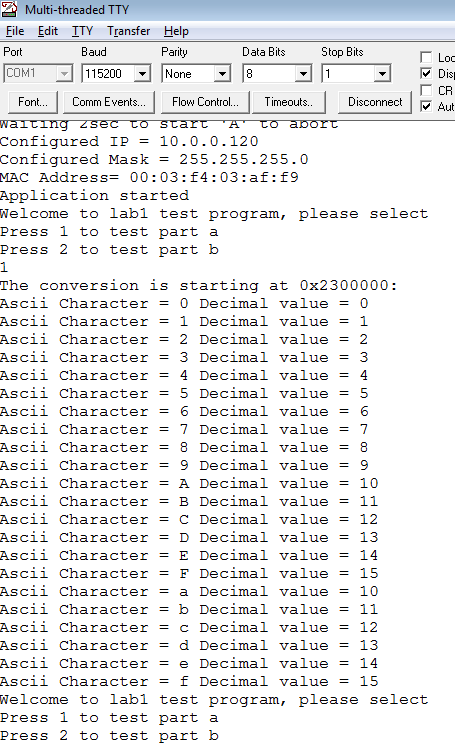
\includegraphics[width=0.4\textwidth]{tst1a.png}
      \caption{MTTTY output when testing our Part A solution}
    \end{figure}

  \subsection{Part B}
    The procedure for testing our code for part B was very similar to the process
    described above in Part A. We visually inspected our code in the Eclipse IDE,
    used the Eclipse debugger to step through our code, and monitor relevant
    memory addresses and registers. When we were confident that we had a working
    solution, we used the provided files \textit{Lab1Test.s}, and the \textit{DataStorage*.s}
    files to verify our solution by downloading the program to the ColdFire microcontroller,
    and monitoring the output in MTTTY. Finally, our solution was verified by a lab TA.

    \begin{figure}[H]
      \centering
      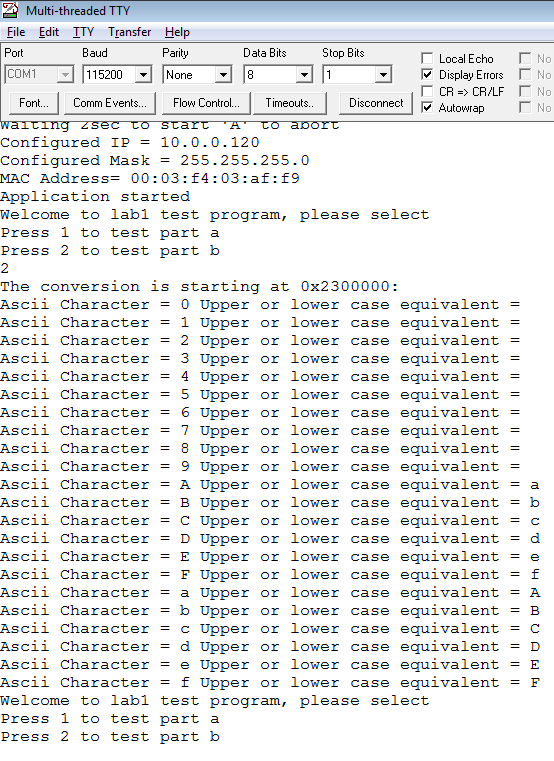
\includegraphics[width=0.4\textwidth]{tst1b.png}
      \caption{MTTTY output when testing our Part B solution}
    \end{figure}

\section{Questions}

    \subsection{Question 1}
      \textit{``What happens when there is no exit code ‘0x0D’ provided in the initialization process? Would it cause a problem? Why or why not?''}
      \\ \\
      \noindent\textbf{A:}
      % \lipsum[7]
      Yes. This would cause a problem, because there would be no way to exit the program,
      so the program would keep reading data and moving the converted values to
      memory locations, until the program attempts to read or write to a memory
      location that is restricted or non-existant. This would then cause the
      program to crash.

    \subsection{Question 2}
      \textit{``How can our code be modified to provide a variable address range? For example, what if I only wanted to convert the first 10 data entires? ''}
      \\ \\
      \noindent\textbf{A:}
      % \lipsum[8]
      Assuming the data range would be fixed and hardcoded into the Assembly code it would be possible to 
      write the max range (ie. 10) into an unused data register such as \%d3.  Then, instead of checking
      for the enter code on each iteration where there is an invalid value, check the value stored in 
      \%d3 before checking the validity of the value stored in the current memory address.  If \%d3 is
      zero then jump to the \textbf{end} label, breaking the loop.  Another way to do it would be again
      to assume that the number of iterations is fixed and the size of data being checked is fixed as being
      long-words would be to check the value of the memory address stored in (\%a1) after each iteration 
      before returning to the beginning of the loop and after the memory addresses have been incremented.  
      If at that point the memory address is [(initial memory address 0x2300000) + (0x4 * N)], where N is
      the number of desired iterations (this value would be hardcoded, this is just a general case), then
      jump to the \textbf{end} label, breaking the loop.  This way would be more memory efficient as it
      does not require an additonal data register and the modification of a counter value.  

\section{Conclusion}
  This lab demonstrated how to use the Assembly language to perform operations
  and modify data while moving it around the ColdFire architechture.  In addition
  the lab improved our understanding of the debugger software, a very powerful
  tool in the development of this kind of code.  The main issue we found was related
  to the hardware itself, as there was some instances where the code did not execute
  properly and the board needed to be reset.  The other issue we faced was mostly 
  around getting used to the software and the workflow in the Eclipse IDE and 
  the debugger.

\newpage
\section{Appendix}
  %\textwidth=600pt
  \subsection{Part A Assembler Code}
    % \begin{changemargin}{-2cm}{-2cm}
    \lstinputlisting{code/parta.s}
  % \end{changemargin}
\newpage
  \subsection{Part A Flowchart Diagram}
    \vspace{2cm}
    \noindent\makebox[\textwidth]{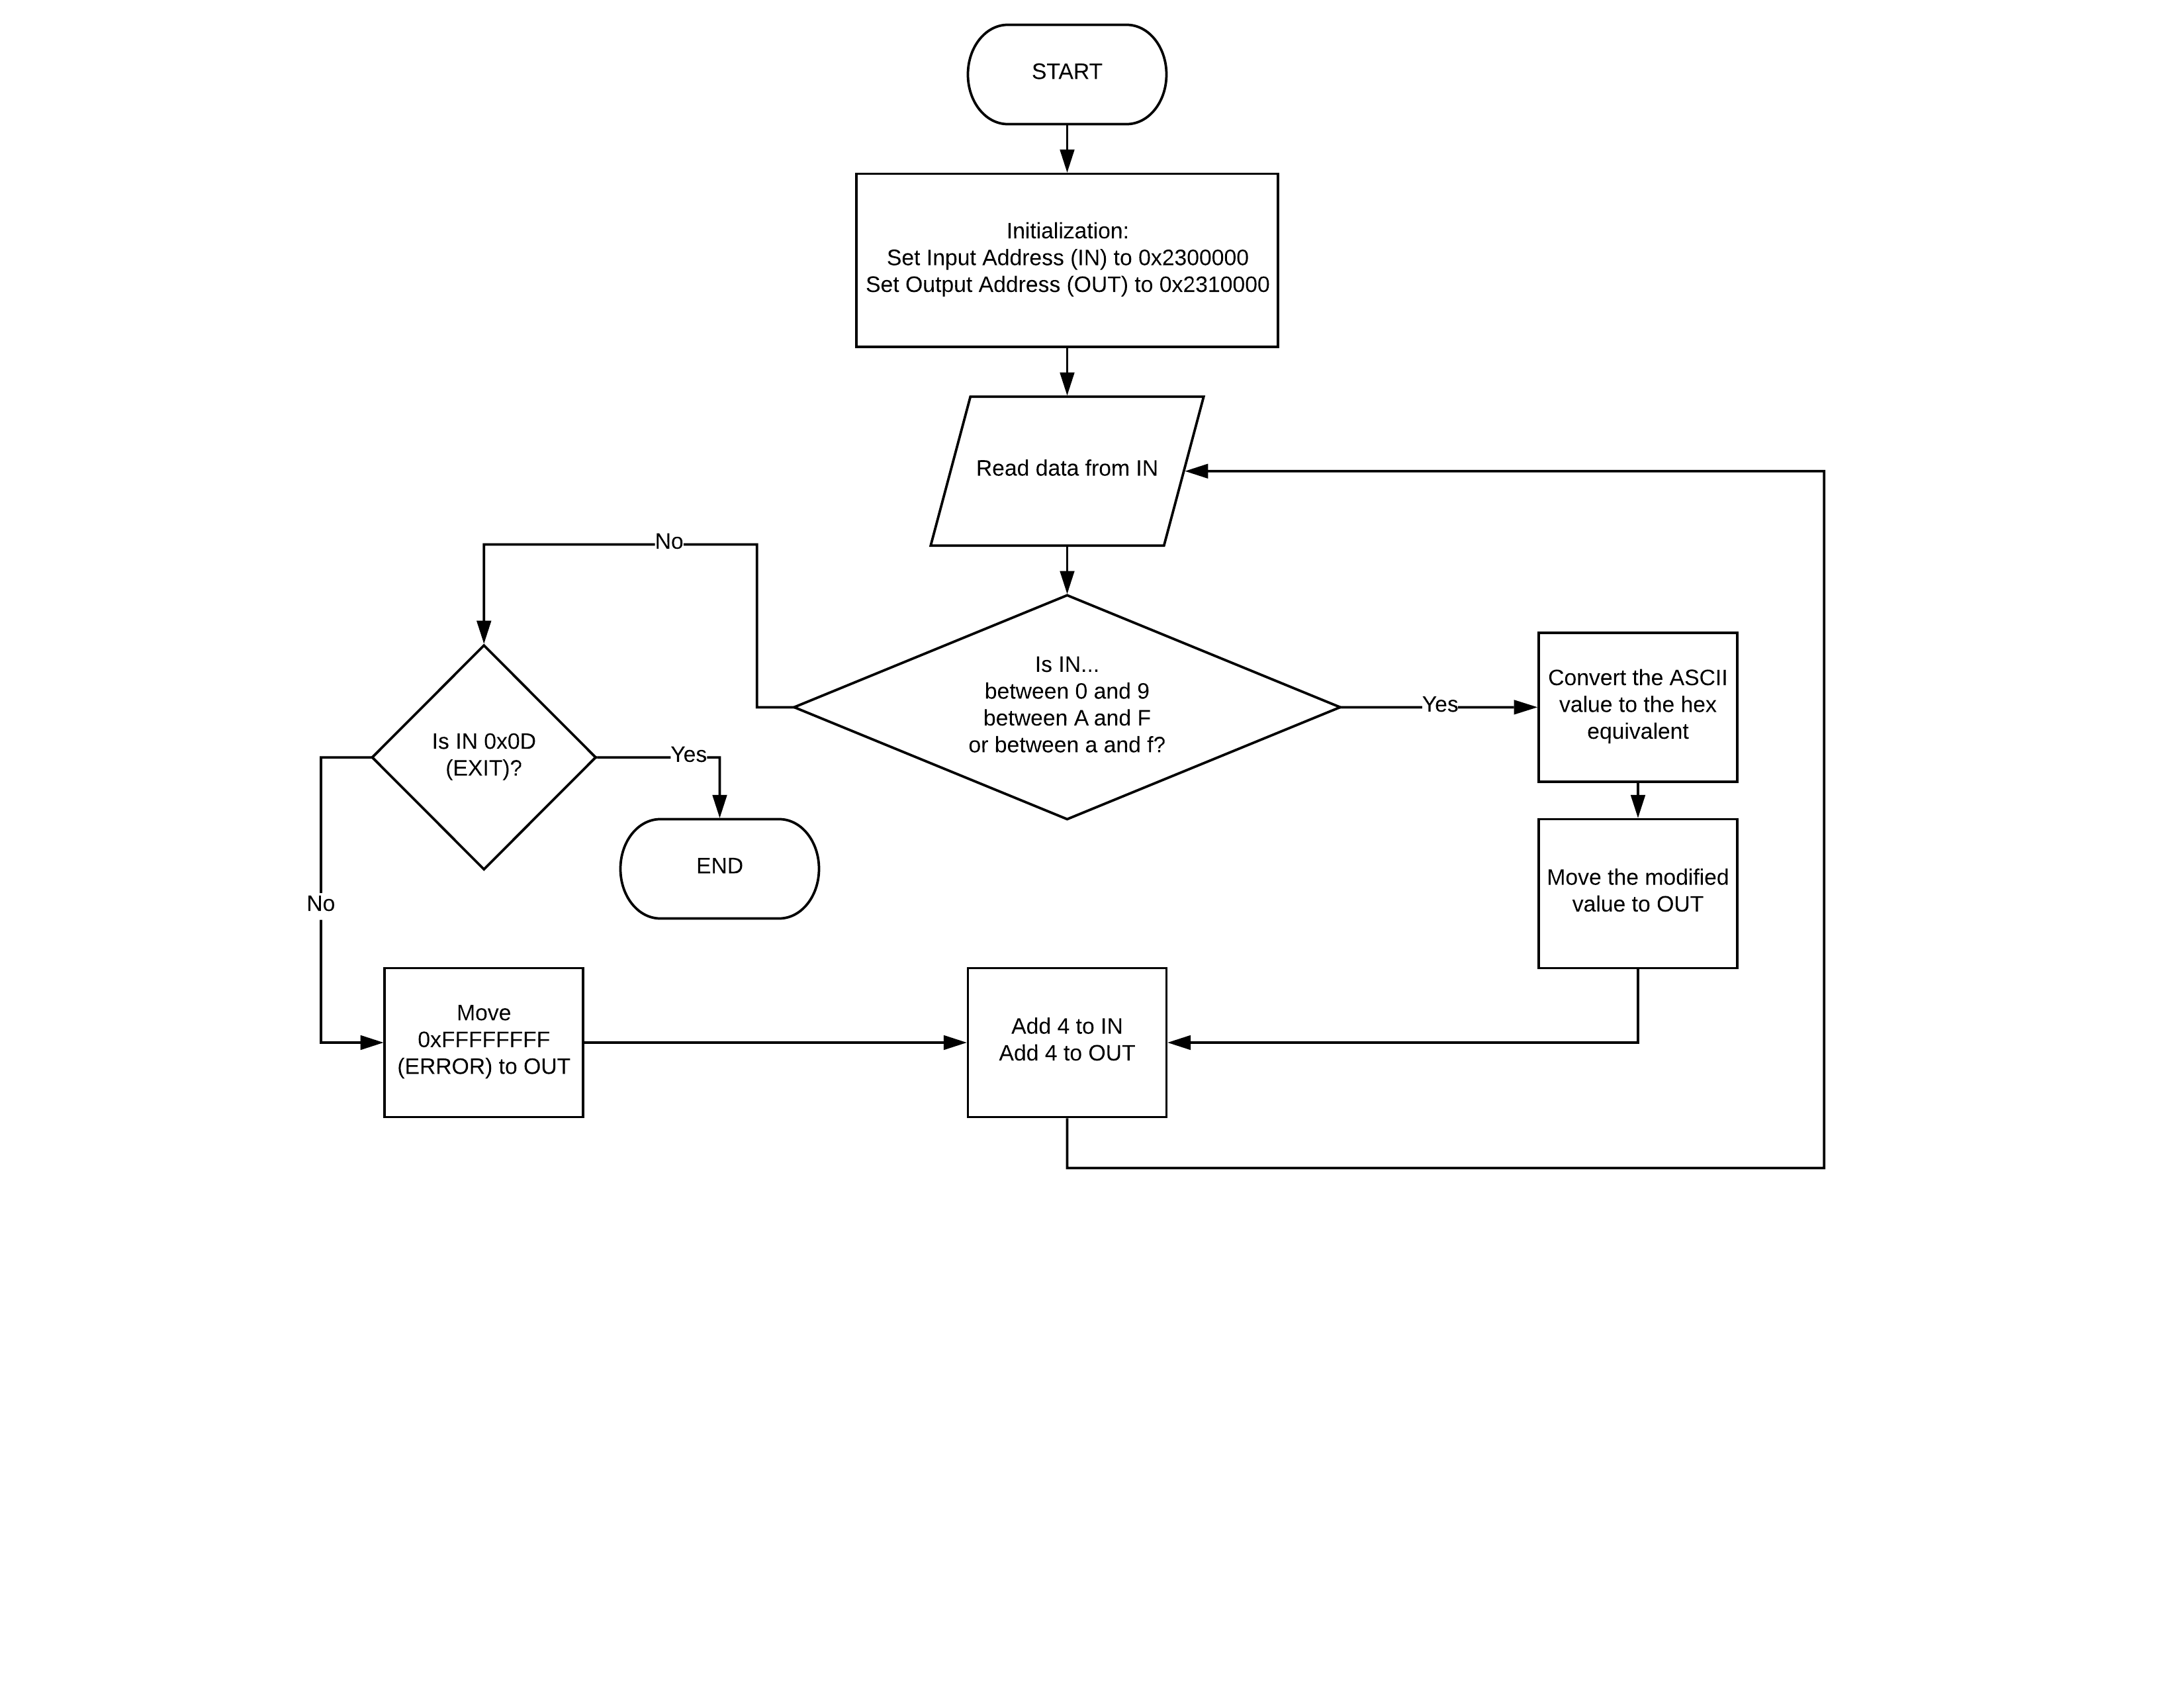
\includegraphics[width=\paperwidth,height=\paperheight,keepaspectratio]{partaflowchart.png}}
\newpage
  \subsection{Part B Assembler Code}
    \lstinputlisting{code/partb.s}
\newpage
  \subsection{Part B Flowchart Diagram}
  \vspace{2cm}
    \noindent\makebox[\textwidth]{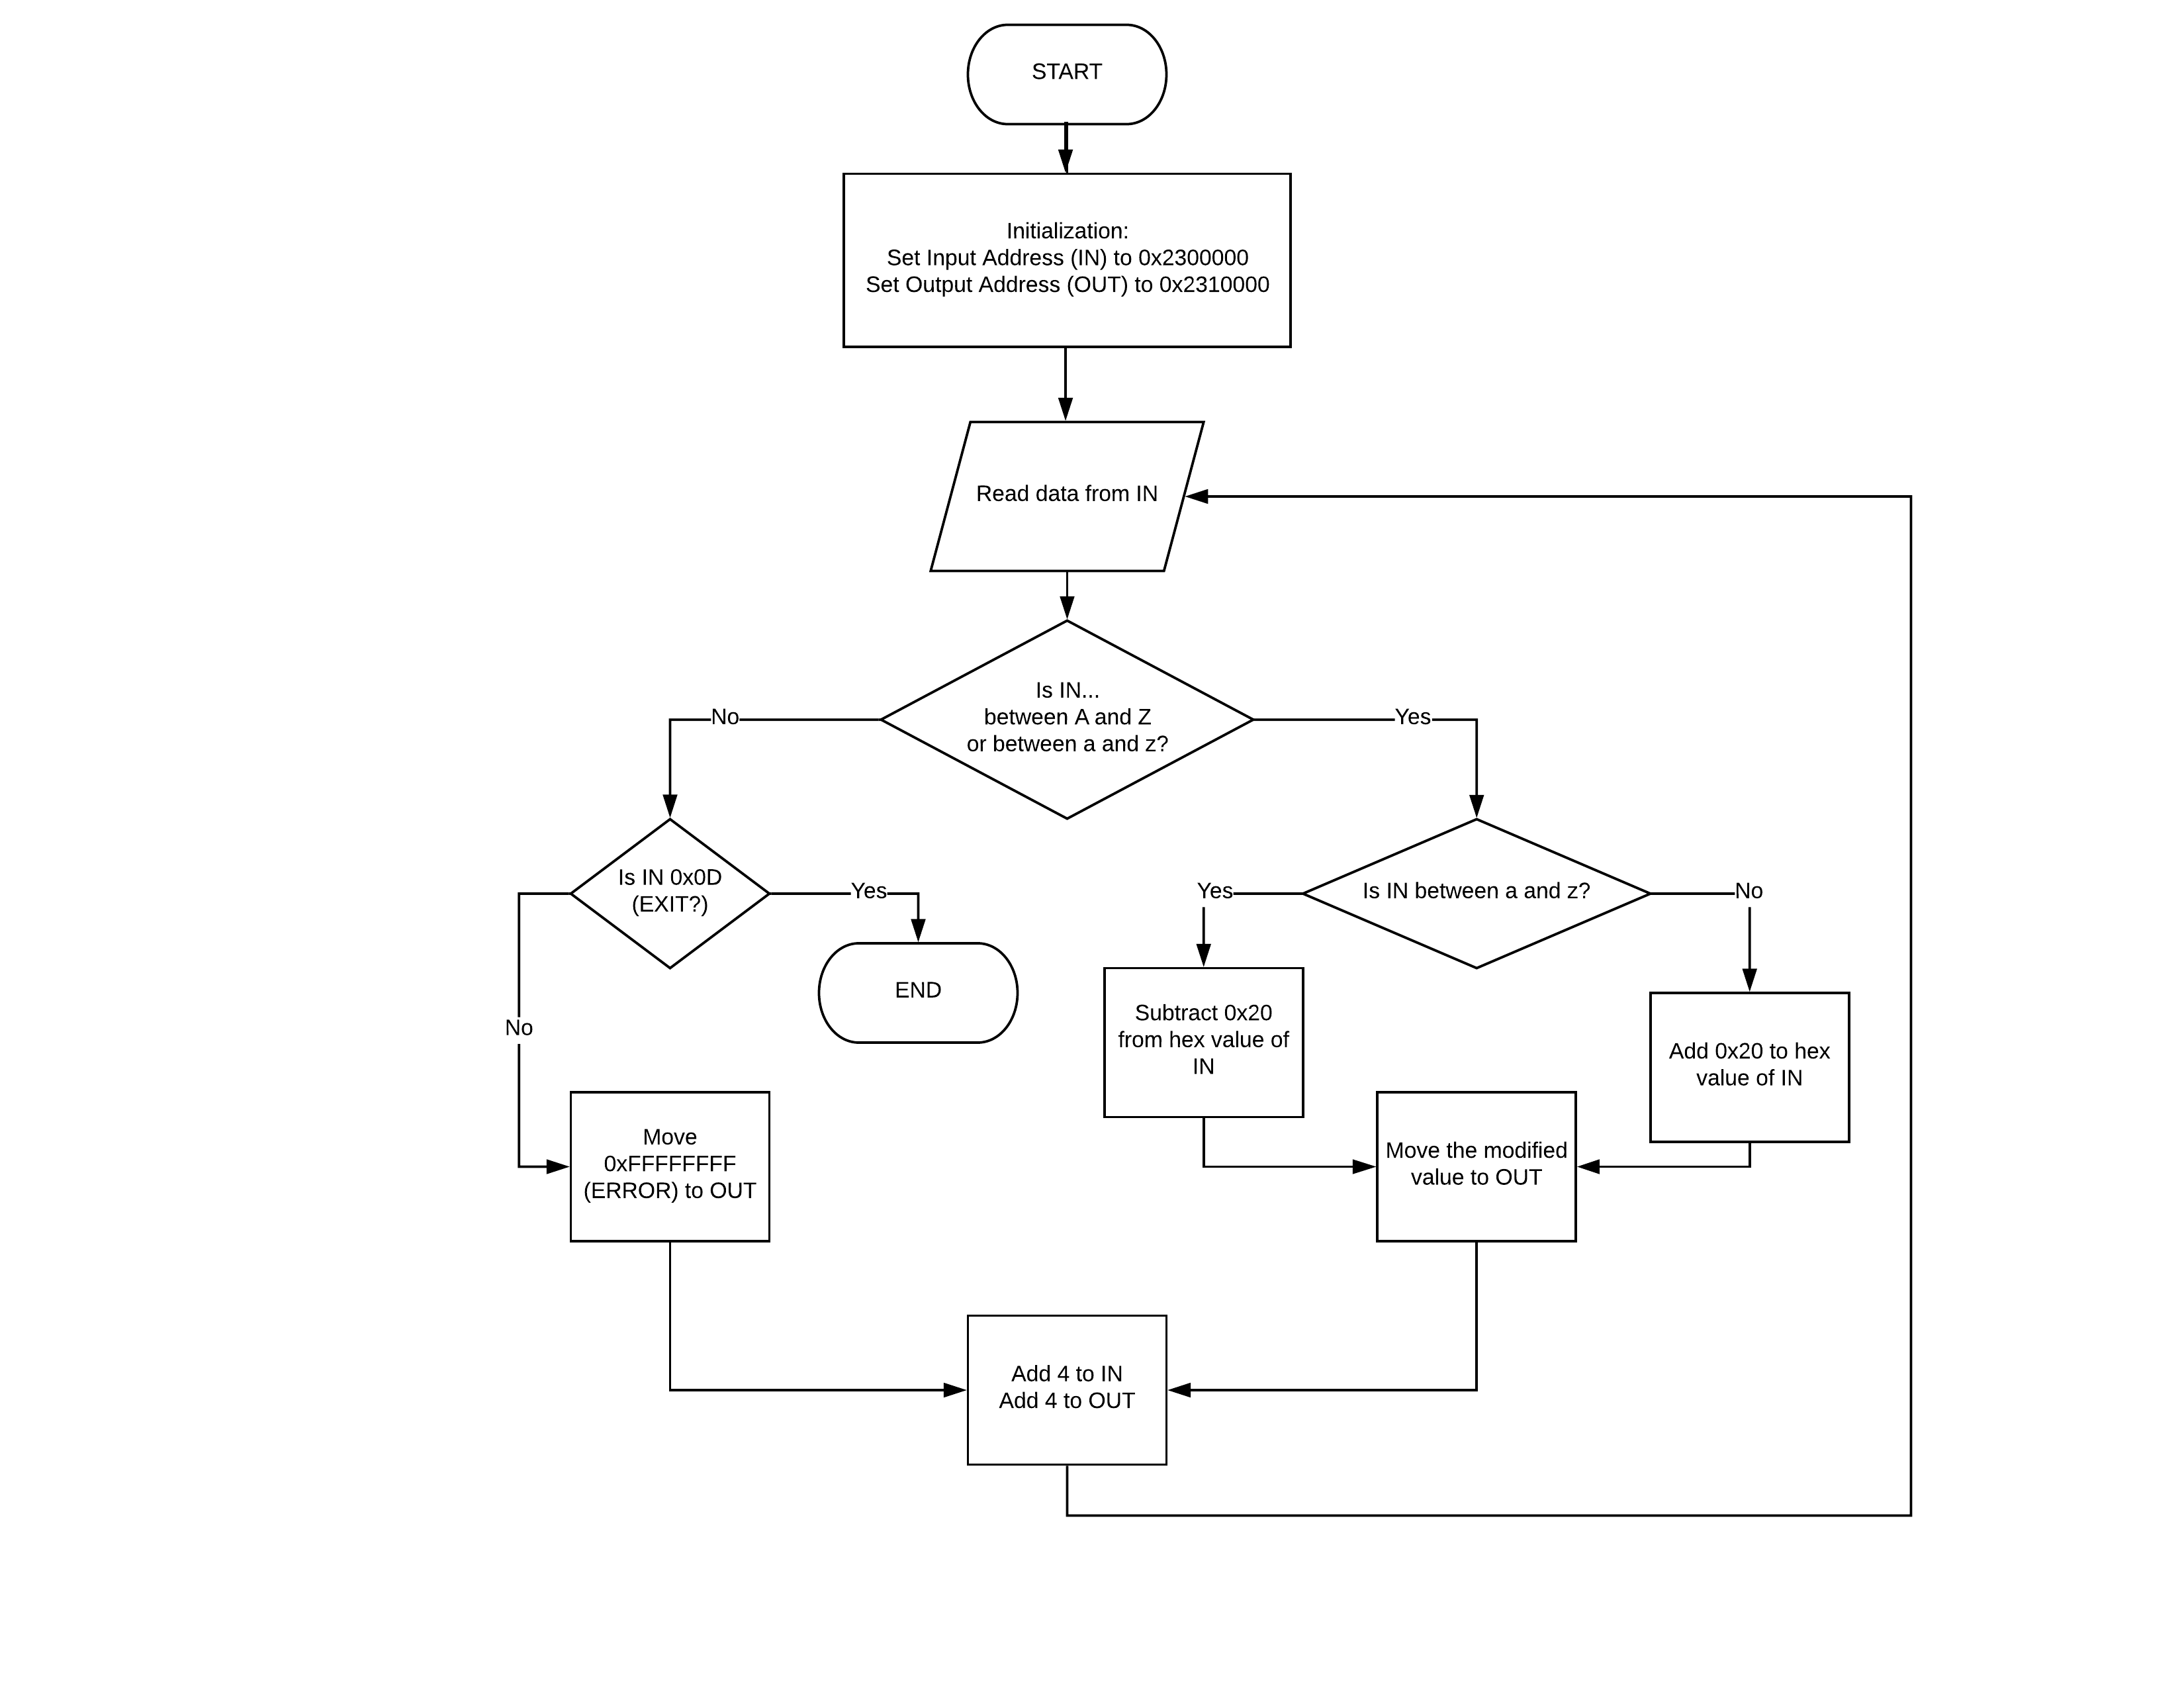
\includegraphics[width=\paperwidth,height=\paperheight,keepaspectratio]{partbflowchart.png}}
\newpage
% \@
% % \pagenumbering{gobble}
% % \addcontentsline{toc}{section}{Marking Sheet}
% % \section{Marking Sheet}
% % \clearpage
% \addtocounter{section}{1}
% % \addcontentsline{toc}{section}{Marking Sheet}
% \addcontentsline{toc}{section}{\protect\numberline{\thesection} Marking Sheet}

\section{Marking Sheet}
\end{document}
